% ------------------------------------------------------------------------------
% TYPO3 CMS 6.2 LTS - What's New (English Version)
% @author Michael Schams <typo3@2013.trash.schams.net>
% @version 1.0.0
%
% ------------------------------------------------------------------------------
% Changelog:
%
% 20 August 2013 - Michael Schams <typo3@2013.trash.schams.net>
%	First initial version
%
% 31 August 2013 - Michael Schams <typo3@2013.trash.schams.net>
%	First two chapters (Introduction and Install Tool) created as proof-of-concept
%
% ------------------------------------------------------------------------------

% change the default aspect ratio and frame size
% \documentclass[aspectratio=43]{beamer}
%
% specify vertical top alignment globally by the [t] class option:
% \documentclass[t]{beamer}
%
% for single frames, use the same option locally:
% \begin{frame}[t] ... \end{frame}

\documentclass[t]{beamer}

% suppress navigation bar
\beamertemplatenavigationsymbolsempty

\mode<presentation>
{
	\usetheme{typo3slides}
}

% global variables
\title{TYPO3 CMS 6.2 LTS - What's New}
\subtitle{Summary of the new features, changes and improvements}
\author{(Author)}
\date{\today}

\begin{document}
%\fontsize{15}{18}\selectfont

% select TYPO3 Share font
\sharefont

% ------------------------------------------------------------------------------
% title page
% ------------------------------------------------------------------------------

\begingroup
	\setbeamercolor{normal text}{fg=white,bg=typo3orange}
	\setbeamercolor{title}{fg=white}
	\setbeamercolor{author}{fg=white}
	\setbeamertemplate{footline}[default]
	\begin{frame}
		\titlepage
	\end{frame}
\endgroup

% ------------------------------------------------------------------------------
% table of contents
% ------------------------------------------------------------------------------

% between two frames: use \newpage (not \clearpage!) to force a column break:
% \addtocontents{toc}{\newpage}

\section*{TYPO3 CMS 6.2 LTS - What's New}
\begin{frame}[fragile]
	\frametitle{Chapter Overview}
	\framesubtitle{Chapter Overview}

	\begin{multicols}{2}
		\tableofcontents
	\end{multicols}

\end{frame}

% ------------------------------------------------------------------------------
% slide
% ------------------------------------------------------------------------------

%\setbeamertemplate{footline}[typo3theme]

\section{Introduction}
\begin{frame}[fragile]
	\frametitle{Introduction}
	\framesubtitle{TYPO3 CMS 6.2 LTS: The Facts}

	\begin{itemize}
		\item Focus on ... *TODO*
		\begin{itemize}
			\item Improving communication
			\item Improving contribution
			\item Improving the product
		\end{itemize}
	\end{itemize}

	\begin{columns}[T]

		\begin{column}{.5\textwidth}
			\begin{itemize}
				\item Release Manager:
				\begin{itemize}
					\item Ernesto Baschny\newline
						benni.mack (at) typo3.org\newline
						@bennimack
				\end{itemize}
			\end{itemize}
		\end{column}

		\begin{column}{.5\textwidth}
%			\begin{figure}
%				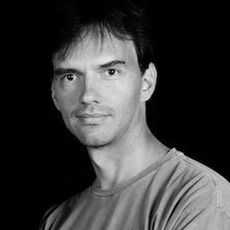
\includegraphics[width=0.6\linewidth]{Images/Introduction/ErnestoBaschny.png}
%			\end{figure}
		\end{column}

	\end{columns}

\end{frame}

% ------------------------------------------------------------------------------
% slide
% ------------------------------------------------------------------------------

\begin{frame}[fragile]
	% \TabPositions{1.2cm}

	\frametitle{Introduction}
	\framesubtitle{TYPO3 CMS 6.2 LTS: The Facts}

	\begin{itemize}
		\item Release date: 30 October 2013
		\item Release timeline:
	\end{itemize}

	\begin{figure}
		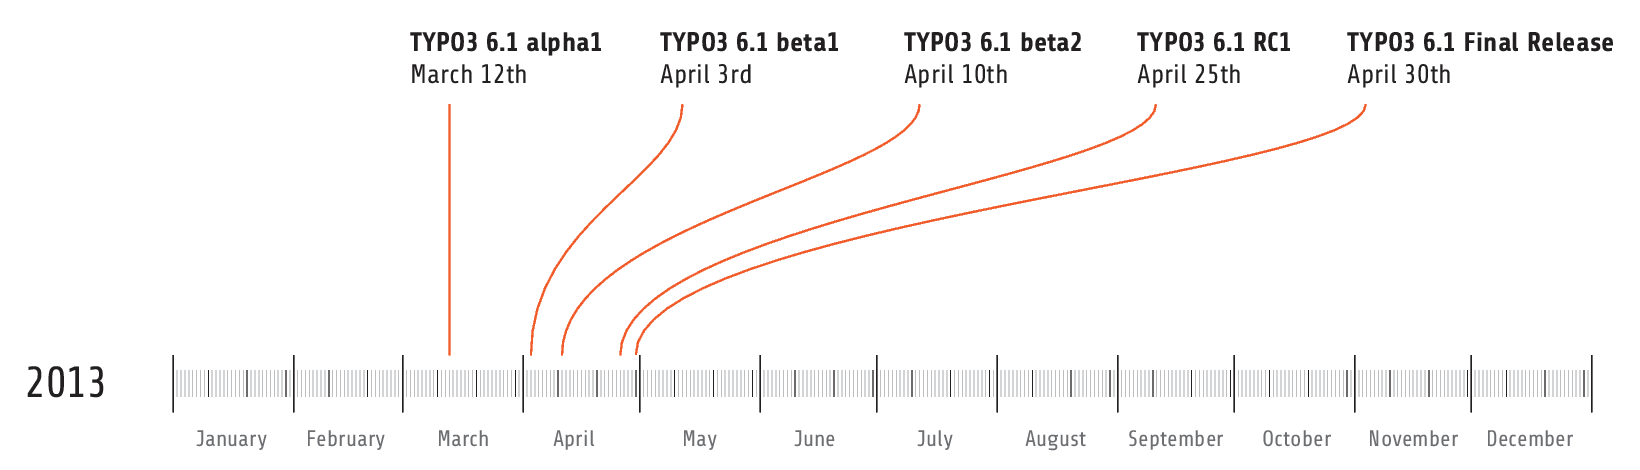
\includegraphics[width=0.99\linewidth]{Images/Introduction/ReleaseTimeline.png}
	\end{figure}

	\begin{itemize}
		\item System Requirements
		\begin{itemize}
			\item PHP	\tabto{1.2cm} v5.3.7 - v5.5.x
			\item MySQL	\tabto{1.2cm} v5.1.x - v5.5.x
		\end{itemize}
	\end{itemize}

\end{frame}

% ------------------------------------------------------------------------------
% slide
% ------------------------------------------------------------------------------

\begin{frame}[fragile]
	\frametitle{Introduction}
	\framesubtitle{TYPO3 CMS 6.2 LTS: The Facts}

	\begin{itemize}
		\item End of maintenance: 30 October 2016 *TODO*\newline
			TYPO3 CMS 6.2 is a \textbf{Long Term Support} (LTS) release!
		\item Release agenda:
	\end{itemize}

%	\begin{figure}
%		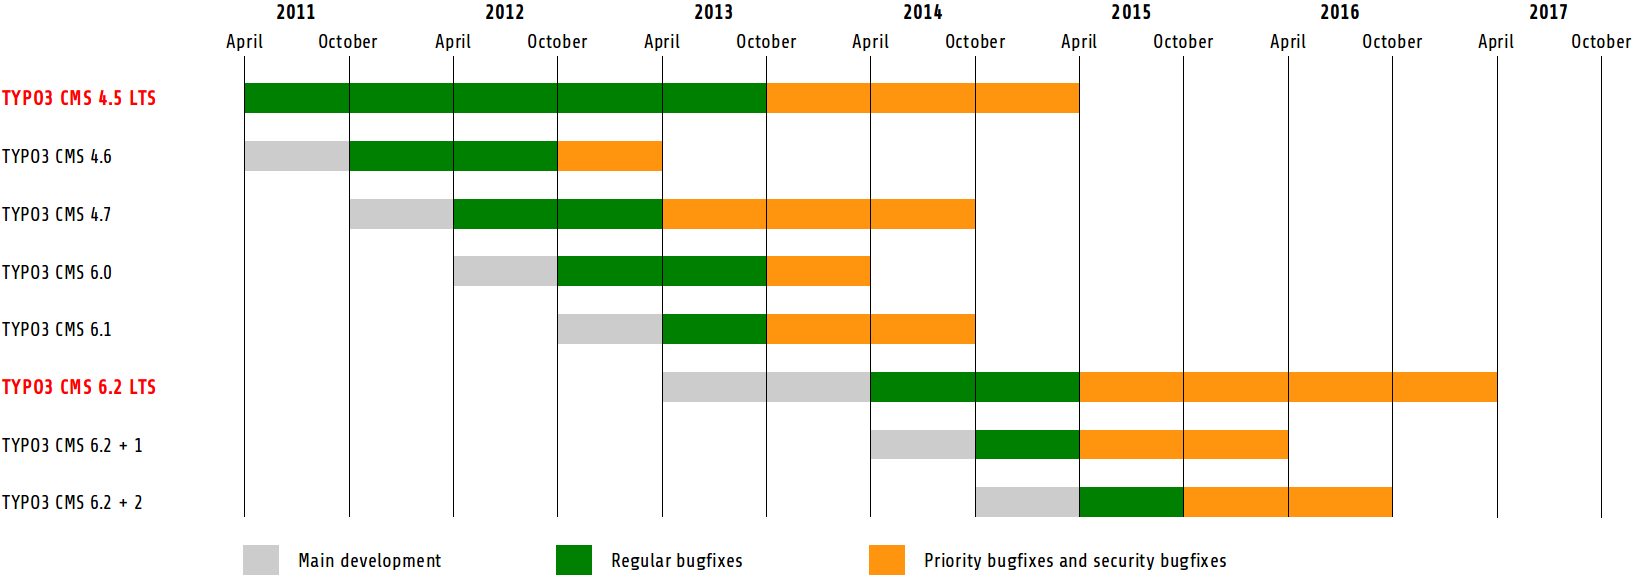
\includegraphics[width=0.6\linewidth]{Images/Introduction/ReleaseAgenda.png}
%	\end{figure}

\end{frame}

% ------------------------------------------------------------------------------
% chapter introduction
% ------------------------------------------------------------------------------

\section{Install Tool}
\begin{frame}[fragile]
	\frametitle{Install Tool}

	\begin{center}\huge{Chapter 1:}\end{center}
	\begin{center}\huge{\color{typo3darkgrey}\textbf{The Install Tool}}\end{center}

\end{frame}

% ------------------------------------------------------------------------------
% slide
% ------------------------------------------------------------------------------

\begin{frame}[fragile]
	\frametitle{Install Tool}
	\framesubtitle{Re-Development}

	\begin{columns}[T]

		\begin{column}{.5\textwidth}
			\begin{itemize}
				\item Re-developed in Extbase/Fluid
				\item \underline{First} step tests system environment and reports issues
				\item reported issues can be fixed\newline
					(and re-tested) or ignored
			\end{itemize}
		\end{column}

		\begin{column}{.5\textwidth}
%			\begin{figure}
%				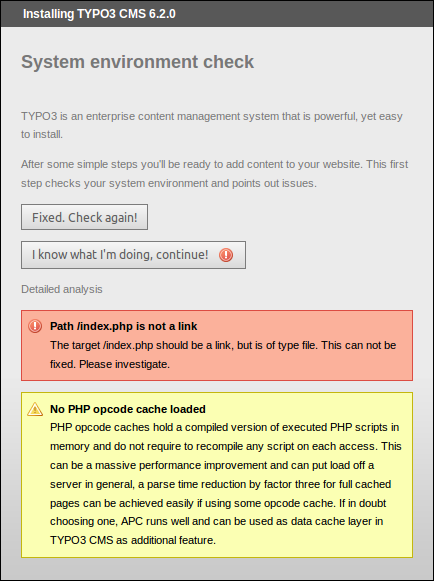
\includegraphics[width=0.6\linewidth]{Images/InstallTool/SystemEnvironmentCheck.png}
%			\end{figure}
		\end{column}

	\end{columns}

\end{frame}

% ------------------------------------------------------------------------------
% slide
% ------------------------------------------------------------------------------

\begin{frame}[fragile]
	\frametitle{Install Tool}
	\framesubtitle{Re-Development}

	\begin{columns}[T]

		\begin{column}{.5\textwidth}
			\begin{itemize}
				\item \underline{Second} step allows users to enter database access details
				\item Connection types are selectable
					\begin{itemize}
						\item TCP/IP based connection
						\item Socket based connection
					\end{itemize}
				\item MySQL alternatives are possible
			\end{itemize}
		\end{column}

		\begin{column}{.5\textwidth}
%			\begin{figure}
%				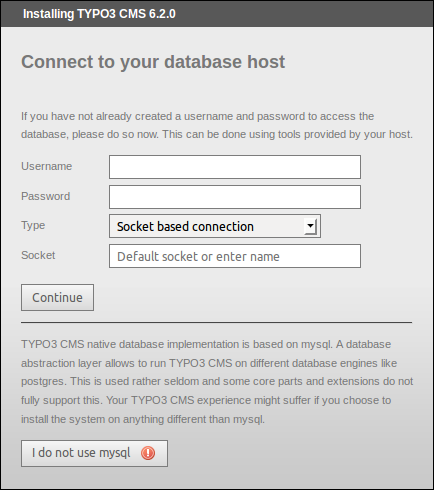
\includegraphics[width=0.6\linewidth]{Images/InstallTool/DatabaseConnectionDetails.png}
%			\end{figure}
		\end{column}

	\end{columns}

\end{frame}

% ------------------------------------------------------------------------------
% slide
% ------------------------------------------------------------------------------

\begin{frame}[fragile]
	\frametitle{Install Tool}
	\framesubtitle{Re-Development}

	\begin{columns}[T]

		\begin{column}{.5\textwidth}
			\begin{itemize}
				\item \underline{Third} step allows users to select/create the database\newline
					(as in versions before TYPO3 6.2)
				\item \underline{Fourth} step allows users to set a password for the "admin" user
				\item ...and a site name
			\end{itemize}
		\end{column}

		\begin{column}{.5\textwidth}
%			\begin{figure}
%				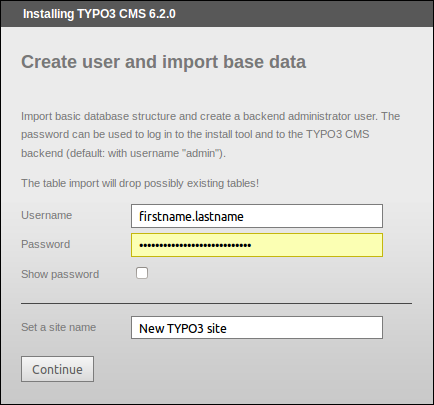
\includegraphics[width=0.6\linewidth]{Images/InstallTool/AdminPasswordAndSiteName.png}
%			\end{figure}
		\end{column}

	\end{columns}

\end{frame}

% ------------------------------------------------------------------------------
% slide
% ------------------------------------------------------------------------------

\begin{frame}[fragile]
	\frametitle{Install Tool}
	\framesubtitle{Delete all cache}

	\begin{itemize}
		\item New function under "Important actions" lets users delete all cache
		\item This also works, if cache contains invalid PHP code\newline
			(which possibly locks TYPO3 CMS)
		\item Bypass a not-working TYPO3 CMS by accessing Install Tool directly:\newline
			\texttt{http://www.yourdomain.com/typo3/install}

	\end{itemize}

%	\begin{figure}
%		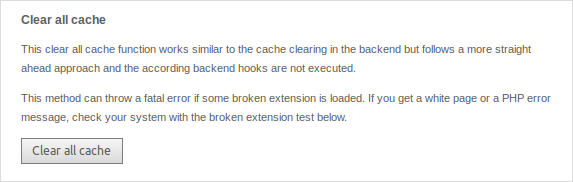
\includegraphics[width=0.6\linewidth]{Images/Introduction/ClearAllCache.png}
%	\end{figure}

\end{frame}

% ------------------------------------------------------------------------------
% slide
% ------------------------------------------------------------------------------

\begin{frame}[fragile]
	\frametitle{Install Tool}
	\framesubtitle{Delete all cache}

	Sequence of actions when executing "Delete all cache":

	\begin{enumerate}
		\item Delete content of directory \texttt{typo3temp/Cache}
		\item Empty database tables \texttt{cf\_*}
		\item Load \texttt{ext\_localconf} and \texttt{ext\_tables} from extensions
		\item Execute \texttt{flushCaches()}
	\end{enumerate}

\end{frame}

% ------------------------------------------------------------------------------
% slide
% ------------------------------------------------------------------------------

\begin{frame}[fragile]
	\frametitle{Install Tool}
	\framesubtitle{Check for broken extensions}

	\begin{itemize}
		\item New function under "Important actions" lets users check,\newline
			if extensions can be loaded without breaking the system
	\end{itemize}

%	\begin{figure}
%		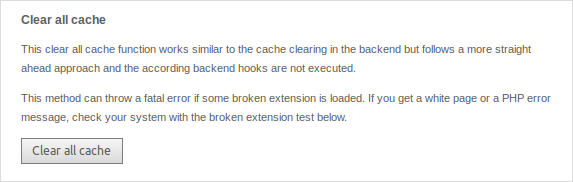
\includegraphics[width=0.6\linewidth]{Images/Introduction/ClearAllCache.png}
%	\end{figure}

\end{frame}

% ------------------------------------------------------------------------------
% slide
% ------------------------------------------------------------------------------

\begin{frame}[fragile]
	\frametitle{Install Tool}
	\framesubtitle{Create backend administrator user}

	\begin{itemize}
		\item When creating new backend administrator user via Install Tool,\newline
			a salted password is used
			(requires installed, loaded and configured EXT:saltedpasswords)
	\end{itemize}

%	\begin{figure}
%		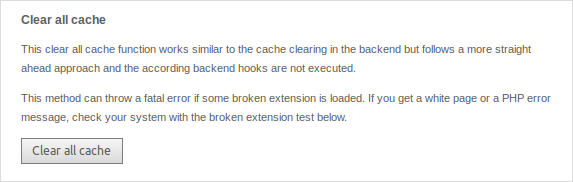
\includegraphics[width=0.6\linewidth]{Images/Introduction/ClearAllCache.png}
%	\end{figure}

\end{frame}

% ------------------------------------------------------------------------------
% slide
% ------------------------------------------------------------------------------

\begin{frame}[fragile]
	% \TabPositions{2cm}

	\frametitle{Install Tool}
	\framesubtitle{Subtitle ???} % *TODO*

	\begin{itemize}
		\item Installer ensures that all required files and directories are in place
		\item Files required for a custom setup will be created automatically
		\item The following symbolic links \underline{must} exist:

		\begin{itemize}
			\item \texttt{typo3\_src}	\tabto{2cm} (points to TYPO3 source directory)
			\item \texttt{typo3}		\tabto{2cm} (points to directory: \texttt{typo3\_src/typo3})
			\item \texttt{index.php}	\tabto{2cm} (points to file: \texttt{typo3\_src/index.php})
		\end{itemize}

		\item No further files/directories are required to install TYPO3!
		\item As a consequence, the TYPO3 Dummy Package becomes obsolute
		\item Further details: see \href{http://docs.typo3.org/typo3cms/InstallationGuide}{TYPO3 Installation and Upgrade Guide}

	\end{itemize}

\end{frame}

% ------------------------------------------------------------------------------
% slide
% ------------------------------------------------------------------------------

\begin{frame}[fragile]
	\frametitle{Install Tool}
	\framesubtitle{Miscellaneous}

	\begin{itemize}
		\item All forms are CSRF (\textit{cross-site request forgery}) protected
		\item Install Tool uses a simplified Fluid Standalone View
		\item Only essential TYPO3 functions are loaded\newline
			(corrupt \texttt{ext\_localconf.php} or \texttt{ext\_tables.php} of extensions can not break the Install Tool any more)
		\item New starting point:	\tabto{3.2cm} \texttt{typo3/sysext/install/Start/Install.php}\newline
			Before:			\tabto{3.2cm} \texttt{typo3/install/index.php}\newline
			(redirect from old to new URL exists)
		\item Deactivated cache ensures that Install Tool remains usable, even if cache contains invalid PHP code
		\item Check if PHP option \texttt{xdebug.max\_nesting\_level} shows a value of 250 or higher (default value "100" possibly causes problems)
	\end{itemize}

\end{frame}

% ------------------------------------------------------------------------------
% chapter introduction
% ------------------------------------------------------------------------------

\section{Test Chapter}
\begin{frame}[fragile]
	\frametitle{Test Chapter}

	\begin{center}\huge{Chapter 2:}\end{center}
	\begin{center}\huge{\color{typo3darkgrey}\textbf{The Test Chapter}}\end{center}

\end{frame}

% ------------------------------------------------------------------------------
% slide
% ------------------------------------------------------------------------------

\begin{frame}
	\frametitle{Test Chapter}
	\framesubtitle{Font Styles}

	\begin{itemize}
		\item \emph{emphasis}
		\item \textsf{Sans}
		\item \texttt{teletypefont}
		\item \textit{italic}
		\item \underline{underline}
		\item \uppercase{uppercase}
		\item \textbf{bold}
		\item \alert{alert}
		\item
			\begingroup
				\color{typo3orange}
				typo3orange
			\endgroup

	\end{itemize}

\end{frame}

% ------------------------------------------------------------------------------
% slide
% ------------------------------------------------------------------------------

\begin{frame}
	\frametitle{Test Chapter}
	\framesubtitle{Links}

	\begin{itemize}
		\item Item
		\item Item with link: \url{http://typo3.org}
		\item Item with \href{http://typo3.org}{link label}

		\item First level
		\begin{itemize}
			\item Second level
			\begin{itemize}
				\item Third level
			\end{itemize}
		\end{itemize}

	\end{itemize}

\end{frame}

% ------------------------------------------------------------------------------
% slide
% ------------------------------------------------------------------------------

\begin{frame}
	\frametitle{Test Chapter}
	\framesubtitle{Item List}

	\begin{itemize}
		\item Item 1
		\item Item 2
		\item Item 3
		\item Item 4
		\item Item 5
		\item Item 6
		\item Item 7
		\item Item 8
		\item Item 9
		\item Item 10
		\item Item 11
		\item Item 12
	\end{itemize}

\end{frame}

% ------------------------------------------------------------------------------

% an empty frame to enforce entries in the table of contents
% *TODO* to be removed later

\section{Empty Frame}
\begin{frame}
\end{frame}

\end{document}

